\documentclass{article}
\usepackage[utf8]{inputenc}
\usepackage[letter, margin=1in]{geometry}
\usepackage{hyperref}
\hypersetup{colorlinks,urlbordercolor=blue,urlcolor=blue,pdfborderstyle={/S/U/W 1}}
\usepackage[colorinlistoftodos]{todonotes}
\title{Middelpos/SAMTEX Notes}
\author{Bob Weigel and Pierre Cilliers}
\date{June 2020}

\usepackage{natbib}
\usepackage{graphicx}

\begin{document}

\todo[inline]{Here's an inline comment.}

\section{Introduction}

Dear Alan,

In the process of documenting results from the South African National Space Agency (SANSA) MT measurements, we came across time series data and transfer function estimates from the SAMTEX project and did a comparison of 

1-second data from LEMI-417M units 

5-second time series MT instrument measurements from ... to ... are from \href{https://www.mtnet.info/data/kap03/kap03.html}{the MT-Solutions KAP03 page}

Second sourcing of the LEMI magnetometers ... \todo{Pierre get instr}

\href{https://www.mtnet.info/data/samtex/samtex.zip}{a zipfile of responses}

%The Laboratory for Electromagnetic Innovations (LEMI) is hereby acknowledged for the use of the  magnetotelluric (MT) processing software made available to SANSA Space Science in Hermanus”.

\href{https://www.mtnet.info/data/samtex/samtex.html}{MT-Solutions SAMTEX page}

\begin{figure}[h!]
\centering
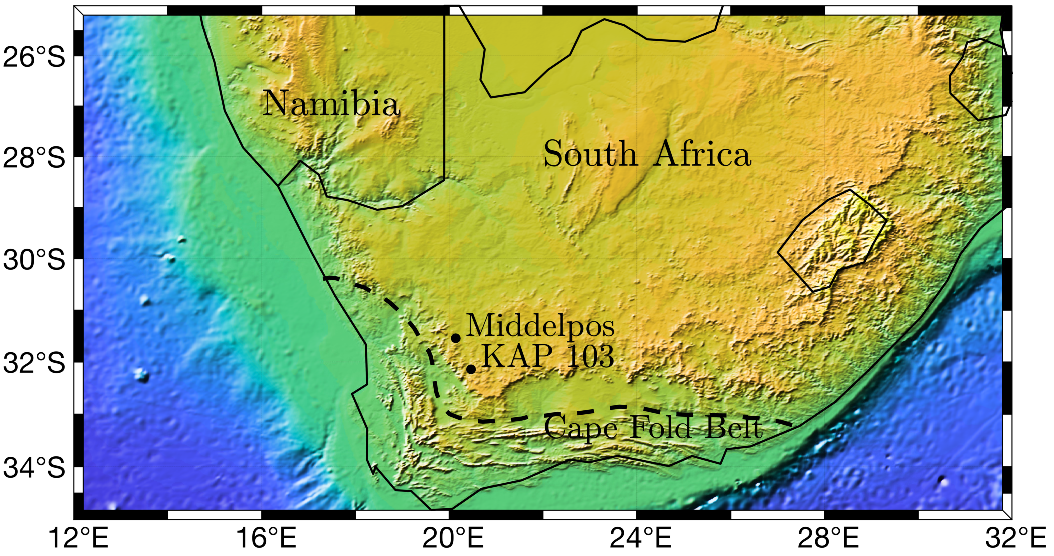
\includegraphics[width=\textwidth]{figures/map.pdf}
\caption{Location of Middelpos [$-31.544^\circ$, $20.141^\circ$] and KAP103 [$-32.139^\circ$, $20.468^\circ$] stations.}
\label{fig:map}
\end{figure}

\clearpage

\section{KAP103 comparison}

\begin{figure}[h!]
\centering
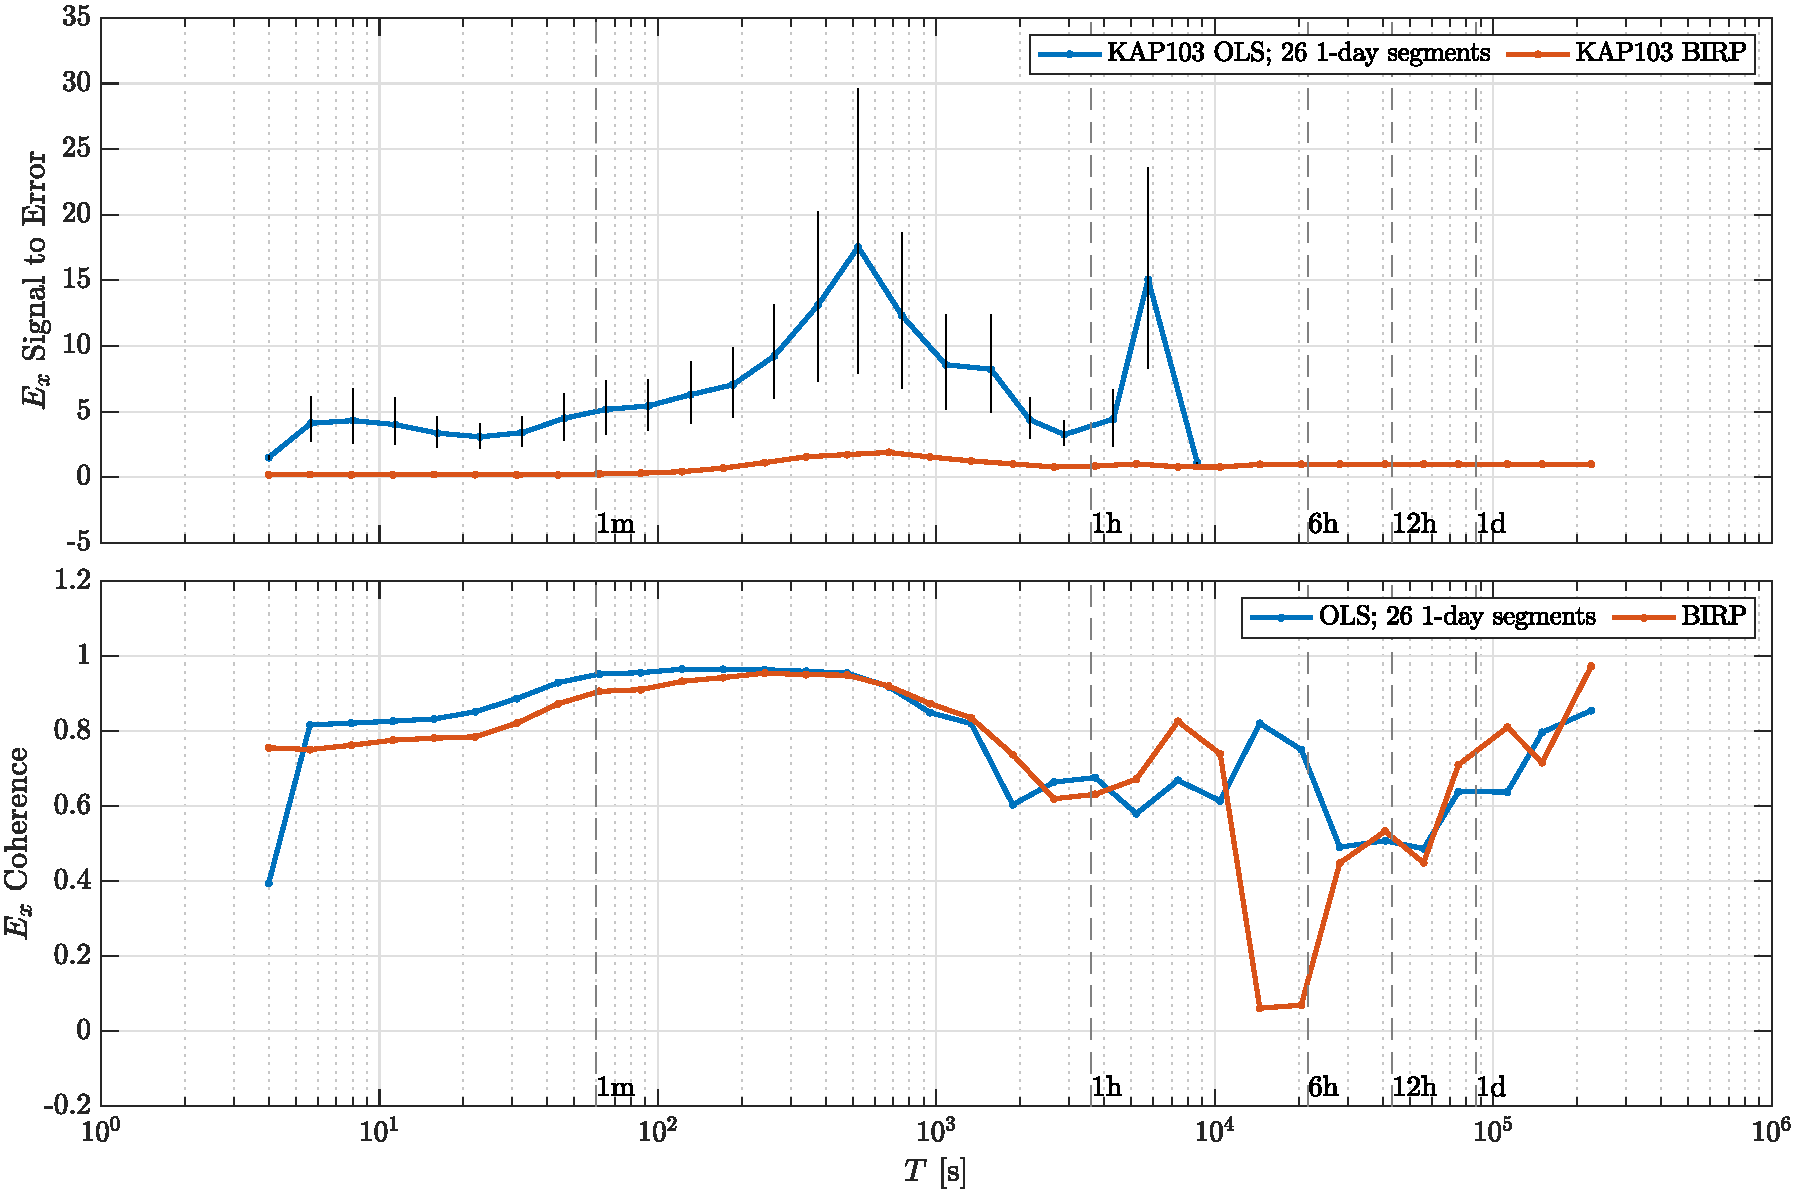
\includegraphics[width=\textwidth]{figures/KAP103/SN_compare-E_x.pdf}
\caption{}
\label{fig:universe}
\end{figure}

\begin{figure}[h!]
\centering
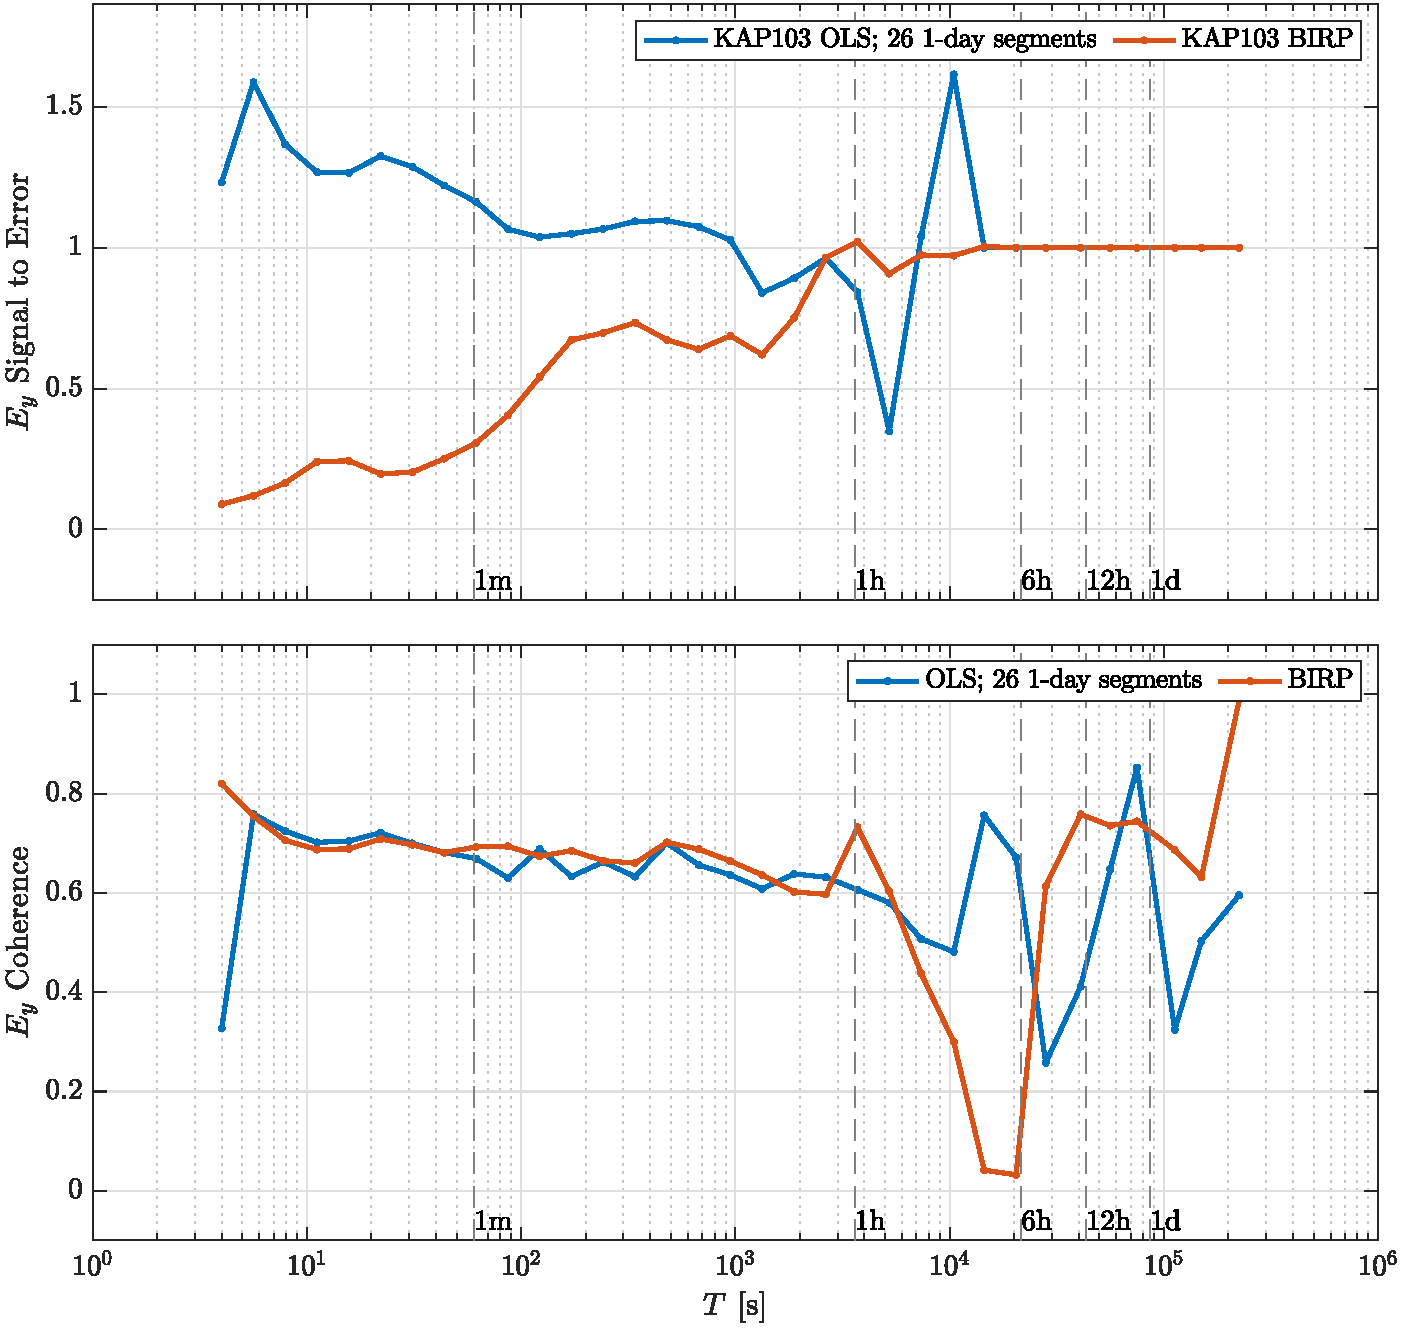
\includegraphics[width=\textwidth]{figures/KAP103/SN_compare-E_y.pdf}
\caption{}
\label{fig:universe}
\end{figure}

\clearpage

\begin{figure}[h!]
\centering
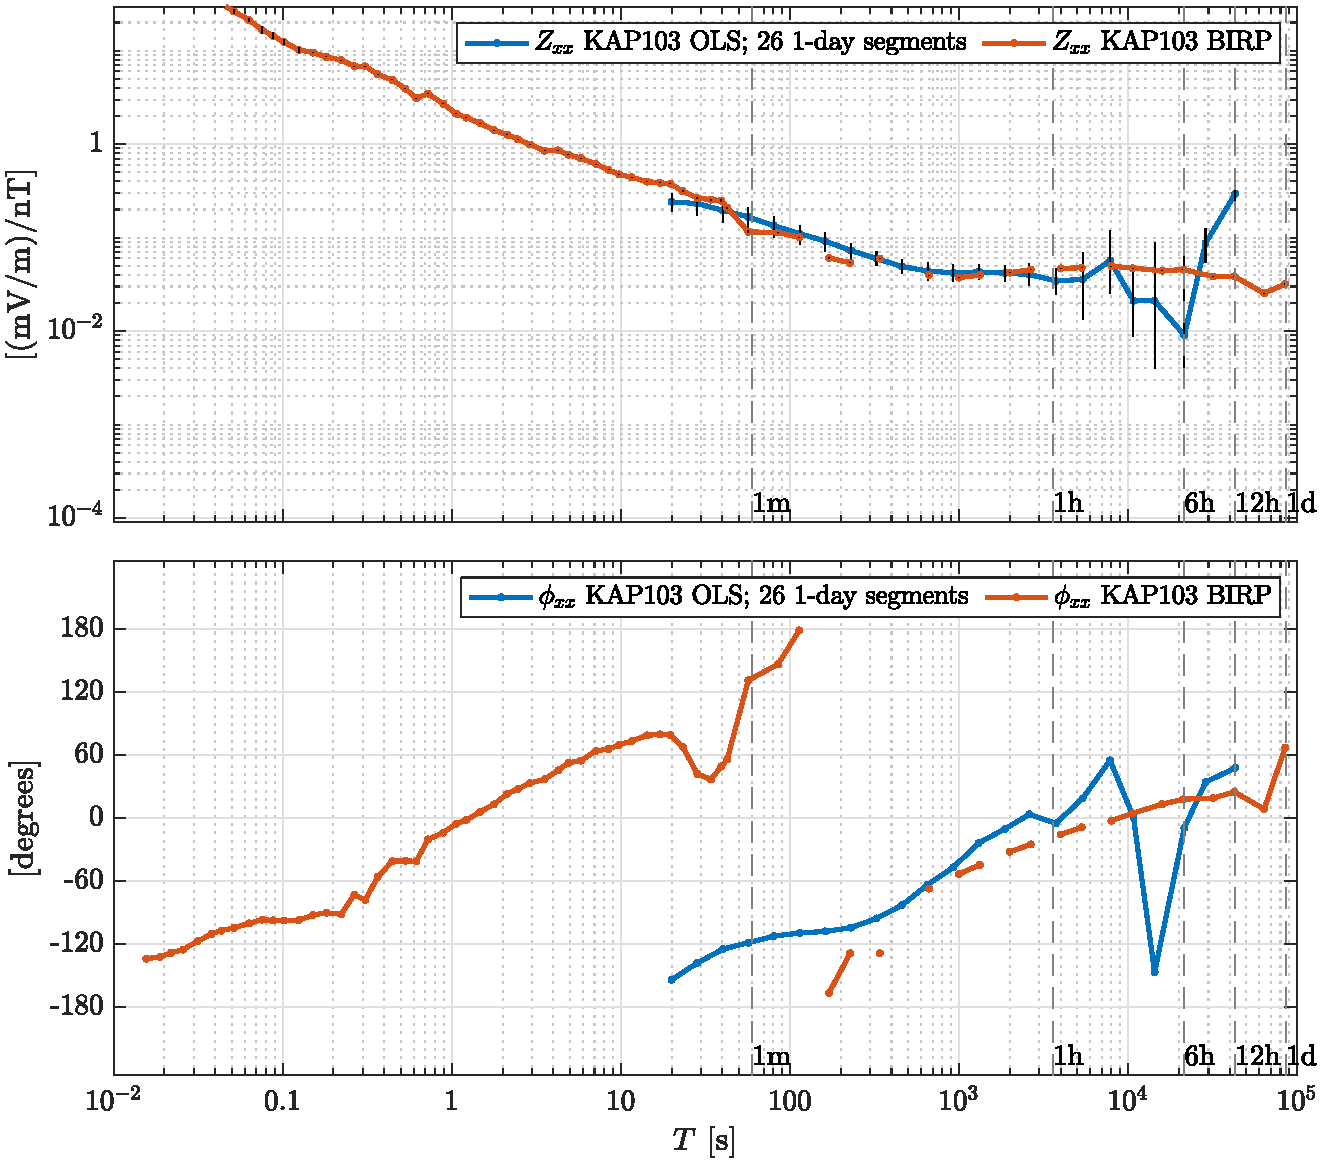
\includegraphics[width=\textwidth]{figures/KAP103/transferfnZ_compare-Z_xx_Magnitude_Phase.pdf}
\caption{}
\end{figure}


\clearpage

\begin{figure}[h!]
\centering
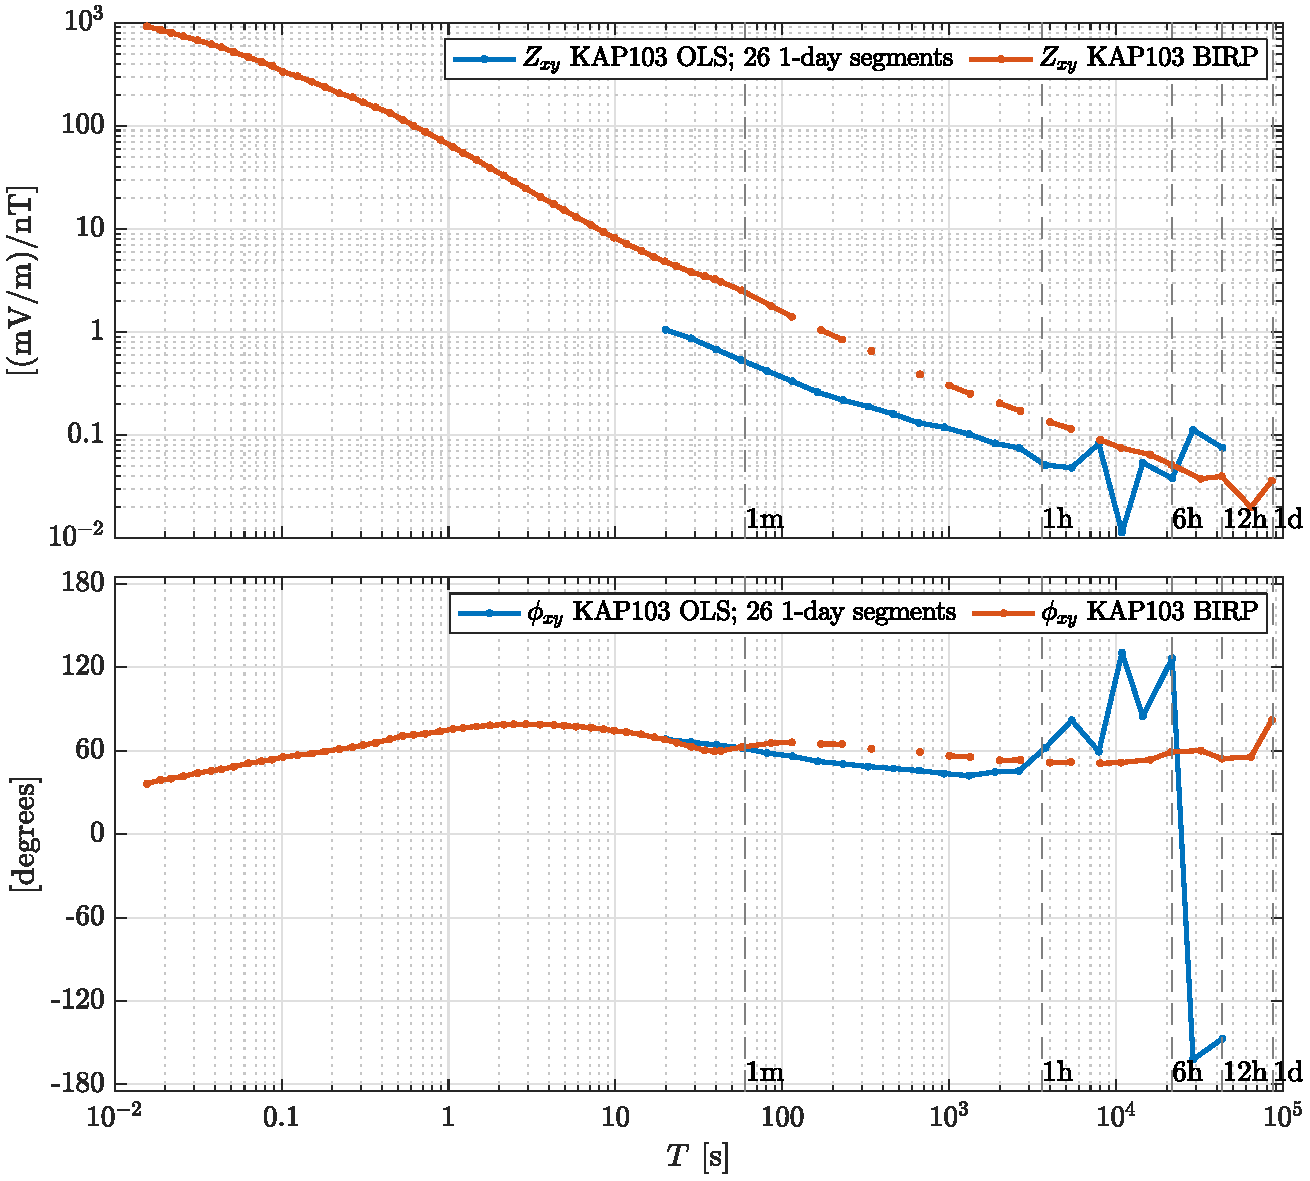
\includegraphics[width=\textwidth]{figures/KAP103/transferfnZ_compare-Z_xy_Magnitude_Phase.pdf}
\caption{}
\label{fig:universe}
\end{figure}

\begin{figure}[h!]
\centering
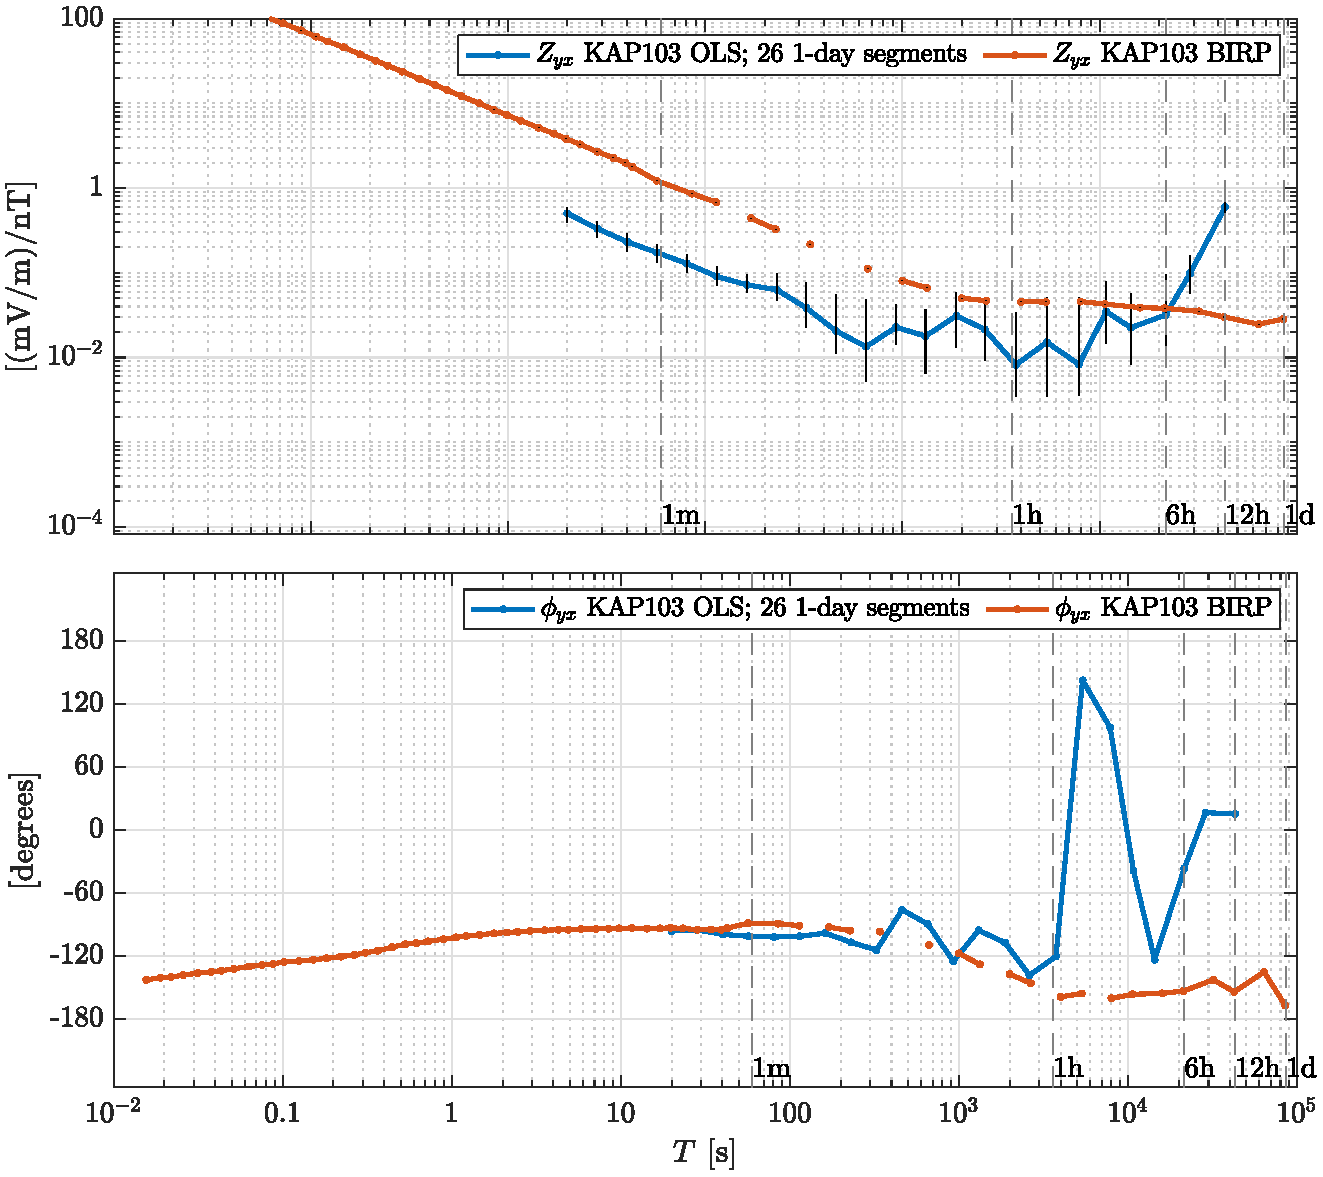
\includegraphics[width=\textwidth]{figures/KAP103/transferfnZ_compare-Z_yx_Magnitude_Phase.pdf}
\caption{}
\label{fig:universe}
\end{figure}

\begin{figure}[h!]
\centering
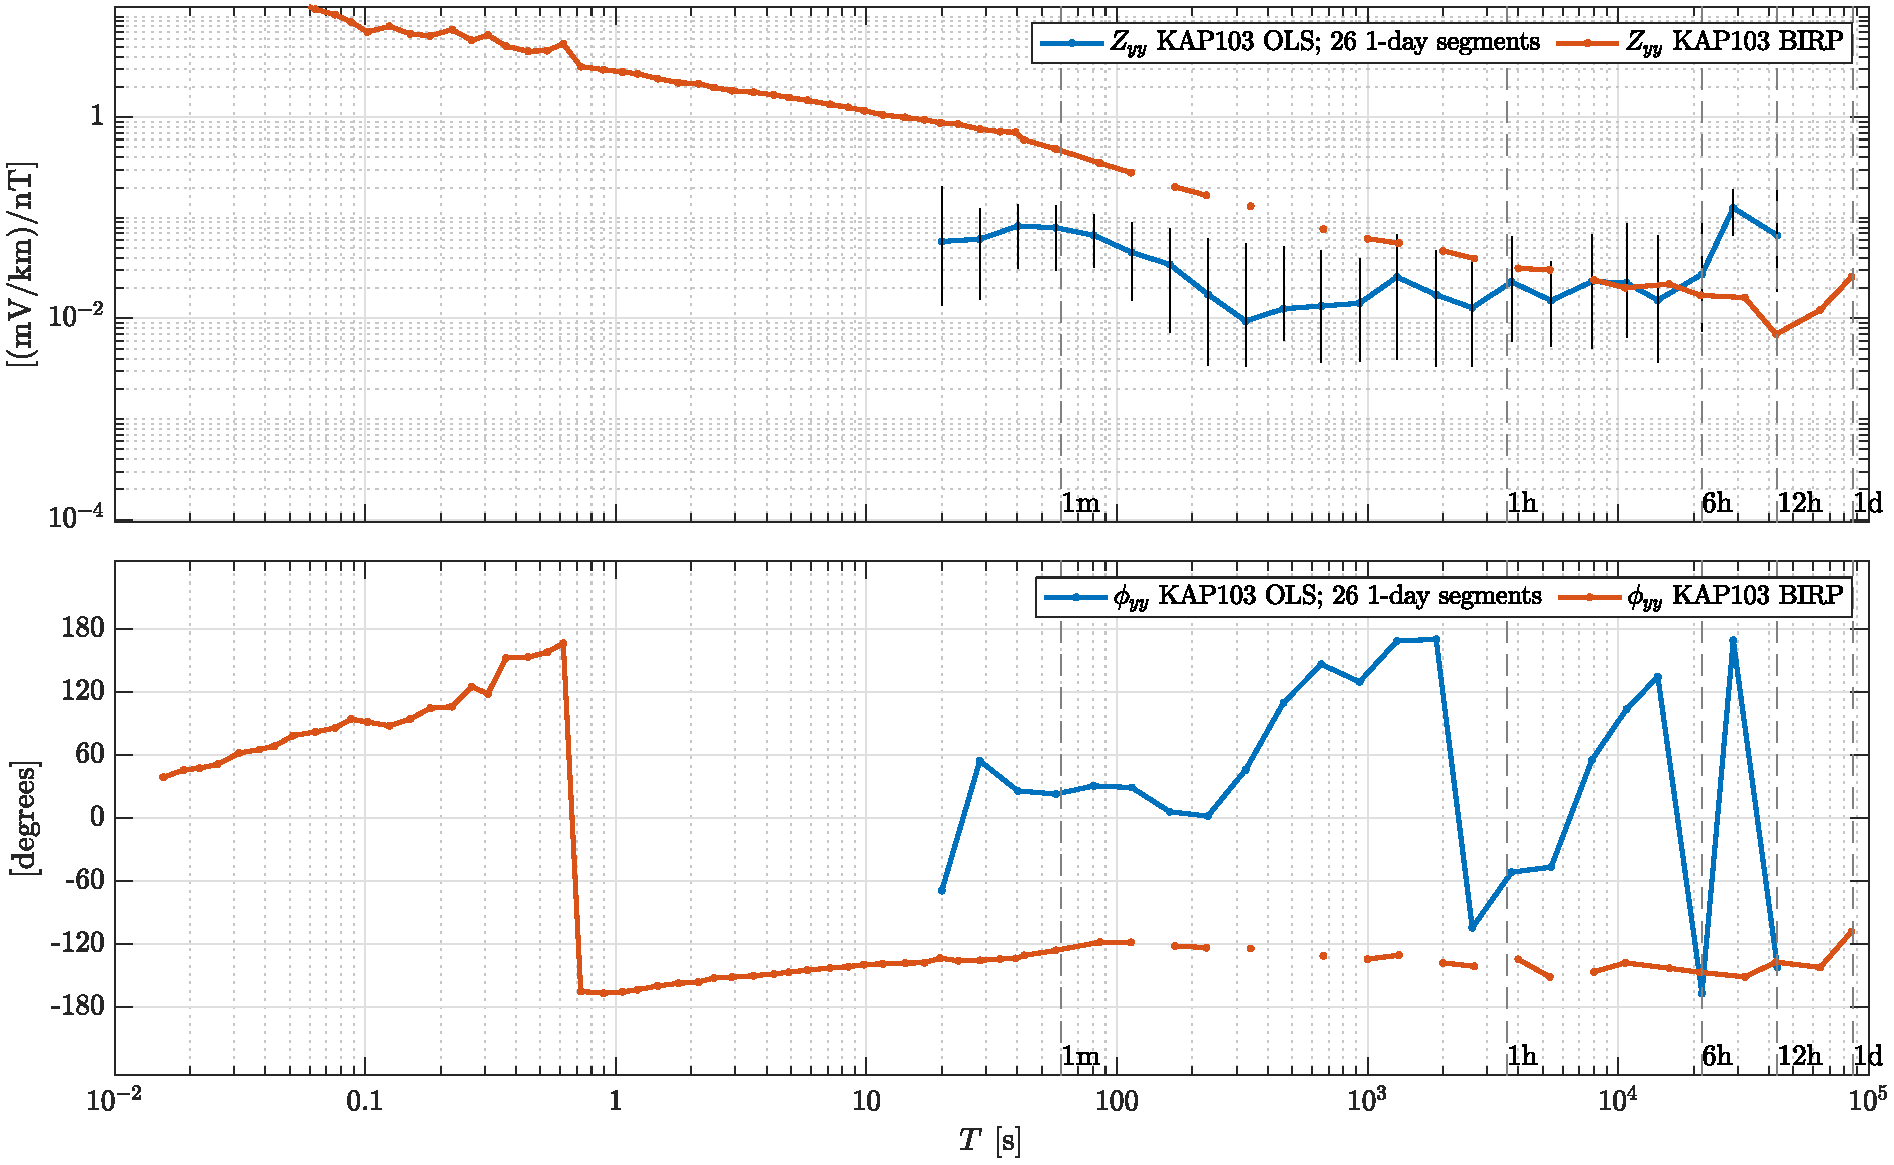
\includegraphics[width=\textwidth]{figures/KAP103/transferfnZ_compare-Z_yy_Magnitude_Phase.pdf}
\caption{}
\label{fig:universe}
\end{figure}

\clearpage

\section{Middelpos/KAP103 comparison}

\begin{figure}[h!]
\centering
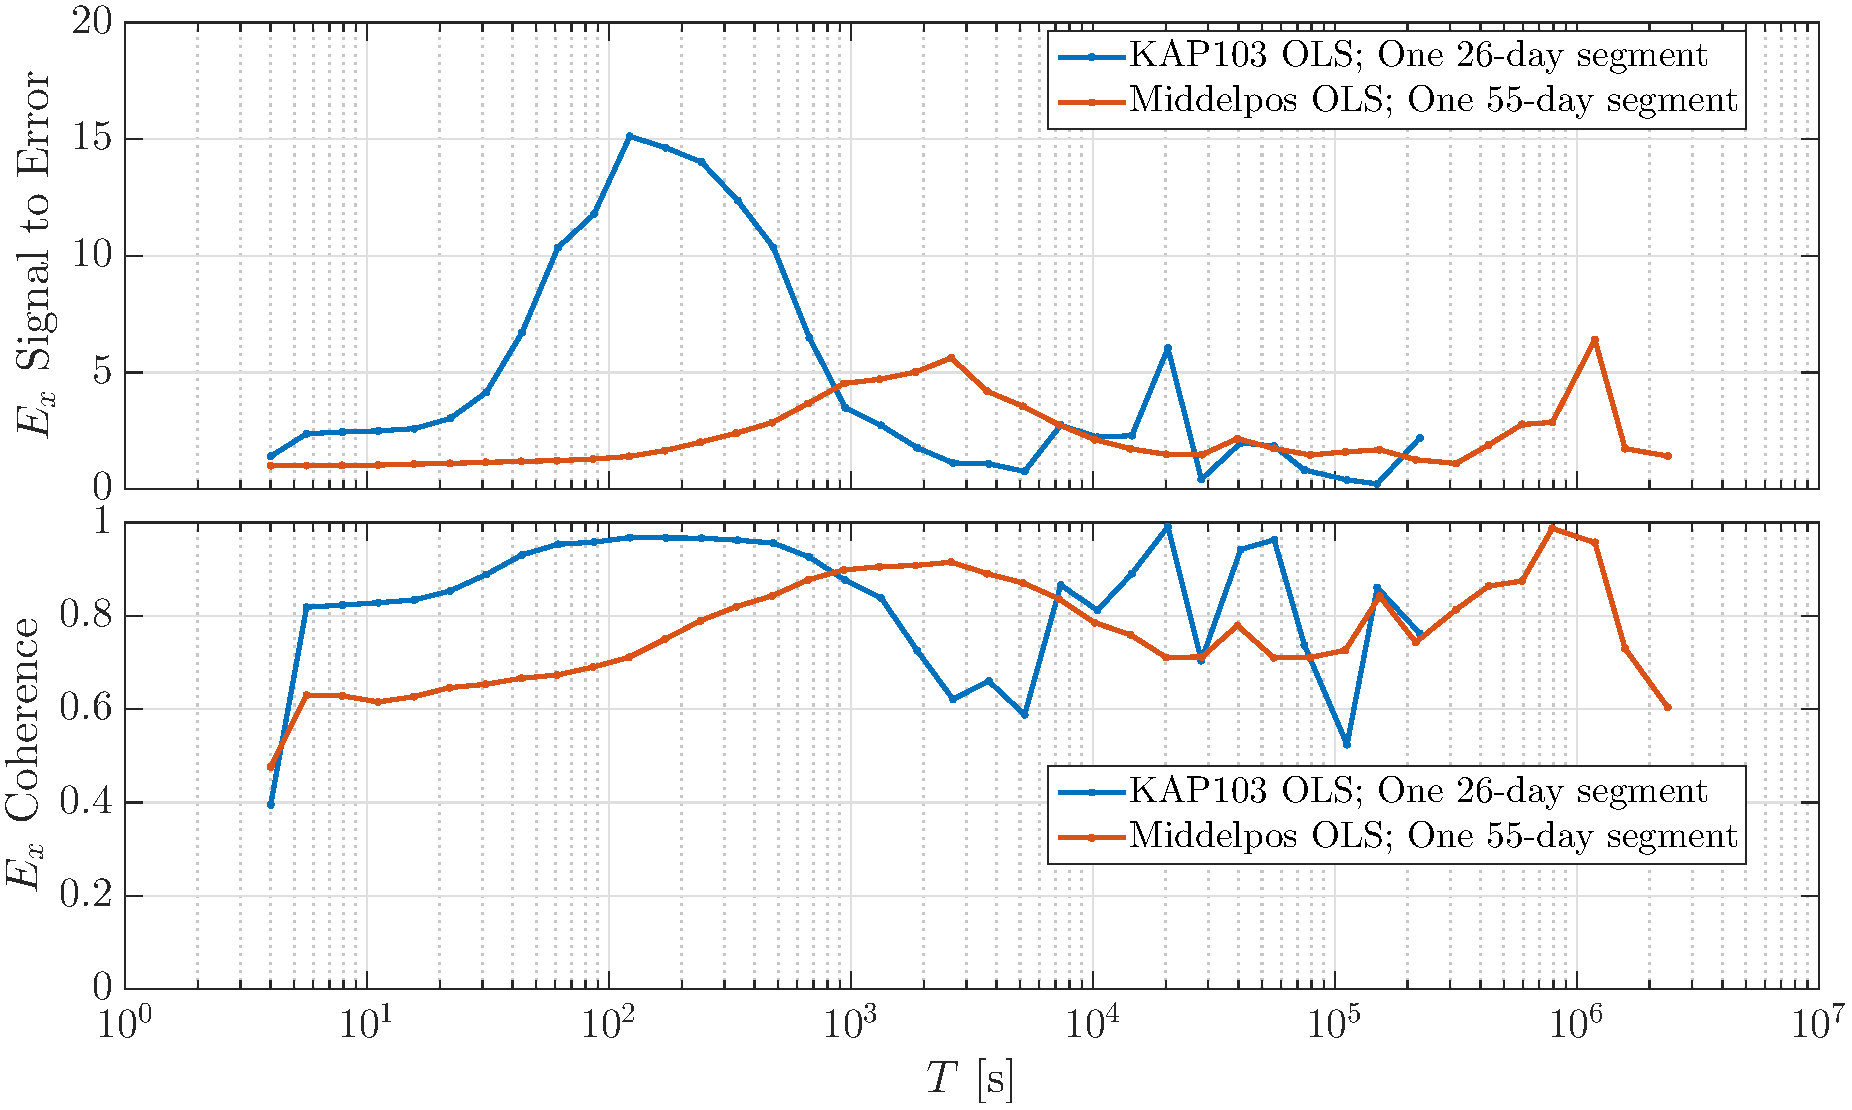
\includegraphics[width=\textwidth]{figures/KAP103_Middelpos/SN-E_x.pdf}
\caption{}
\label{fig:universe}
\end{figure}

\begin{figure}[h!]
\centering
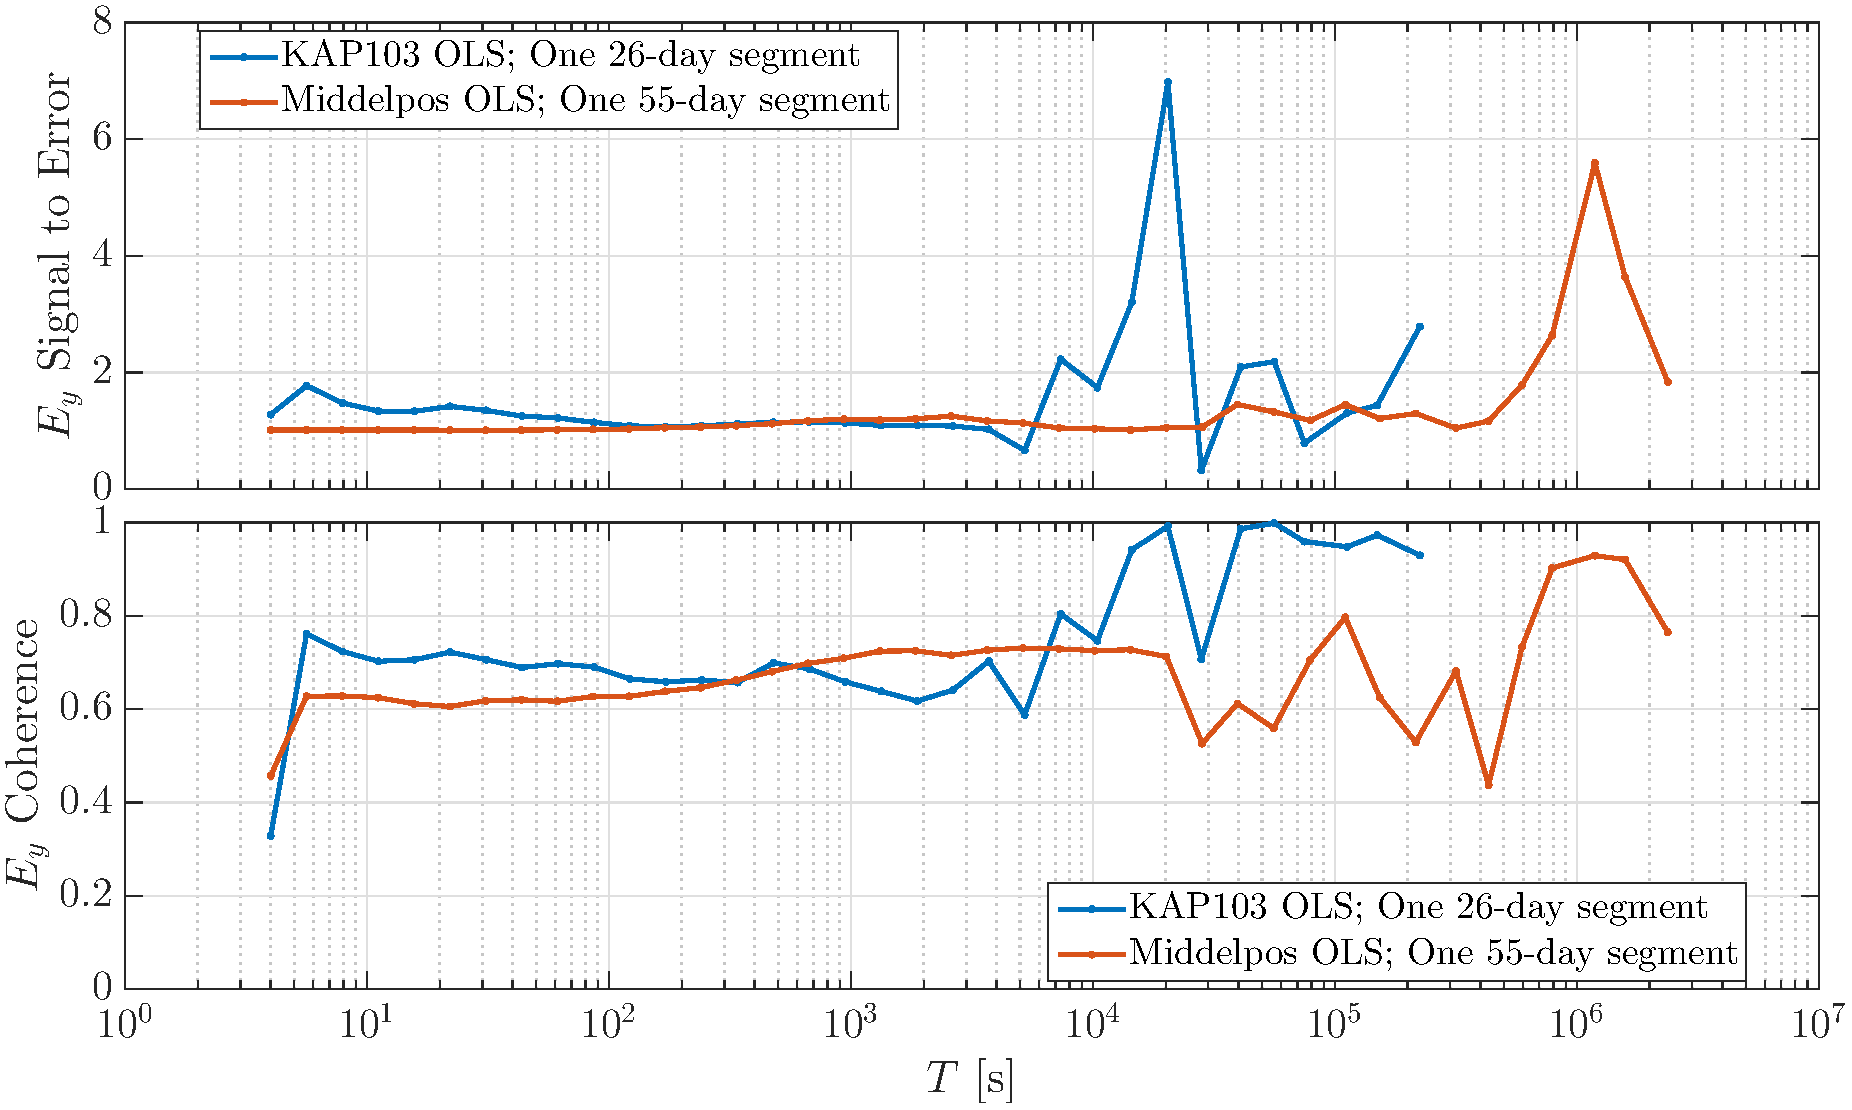
\includegraphics[width=\textwidth]{figures/KAP103_Middelpos/SN-E_y.pdf}
\caption{}
\label{fig:universe}
\end{figure}

\clearpage

\begin{figure}[h!]
\centering
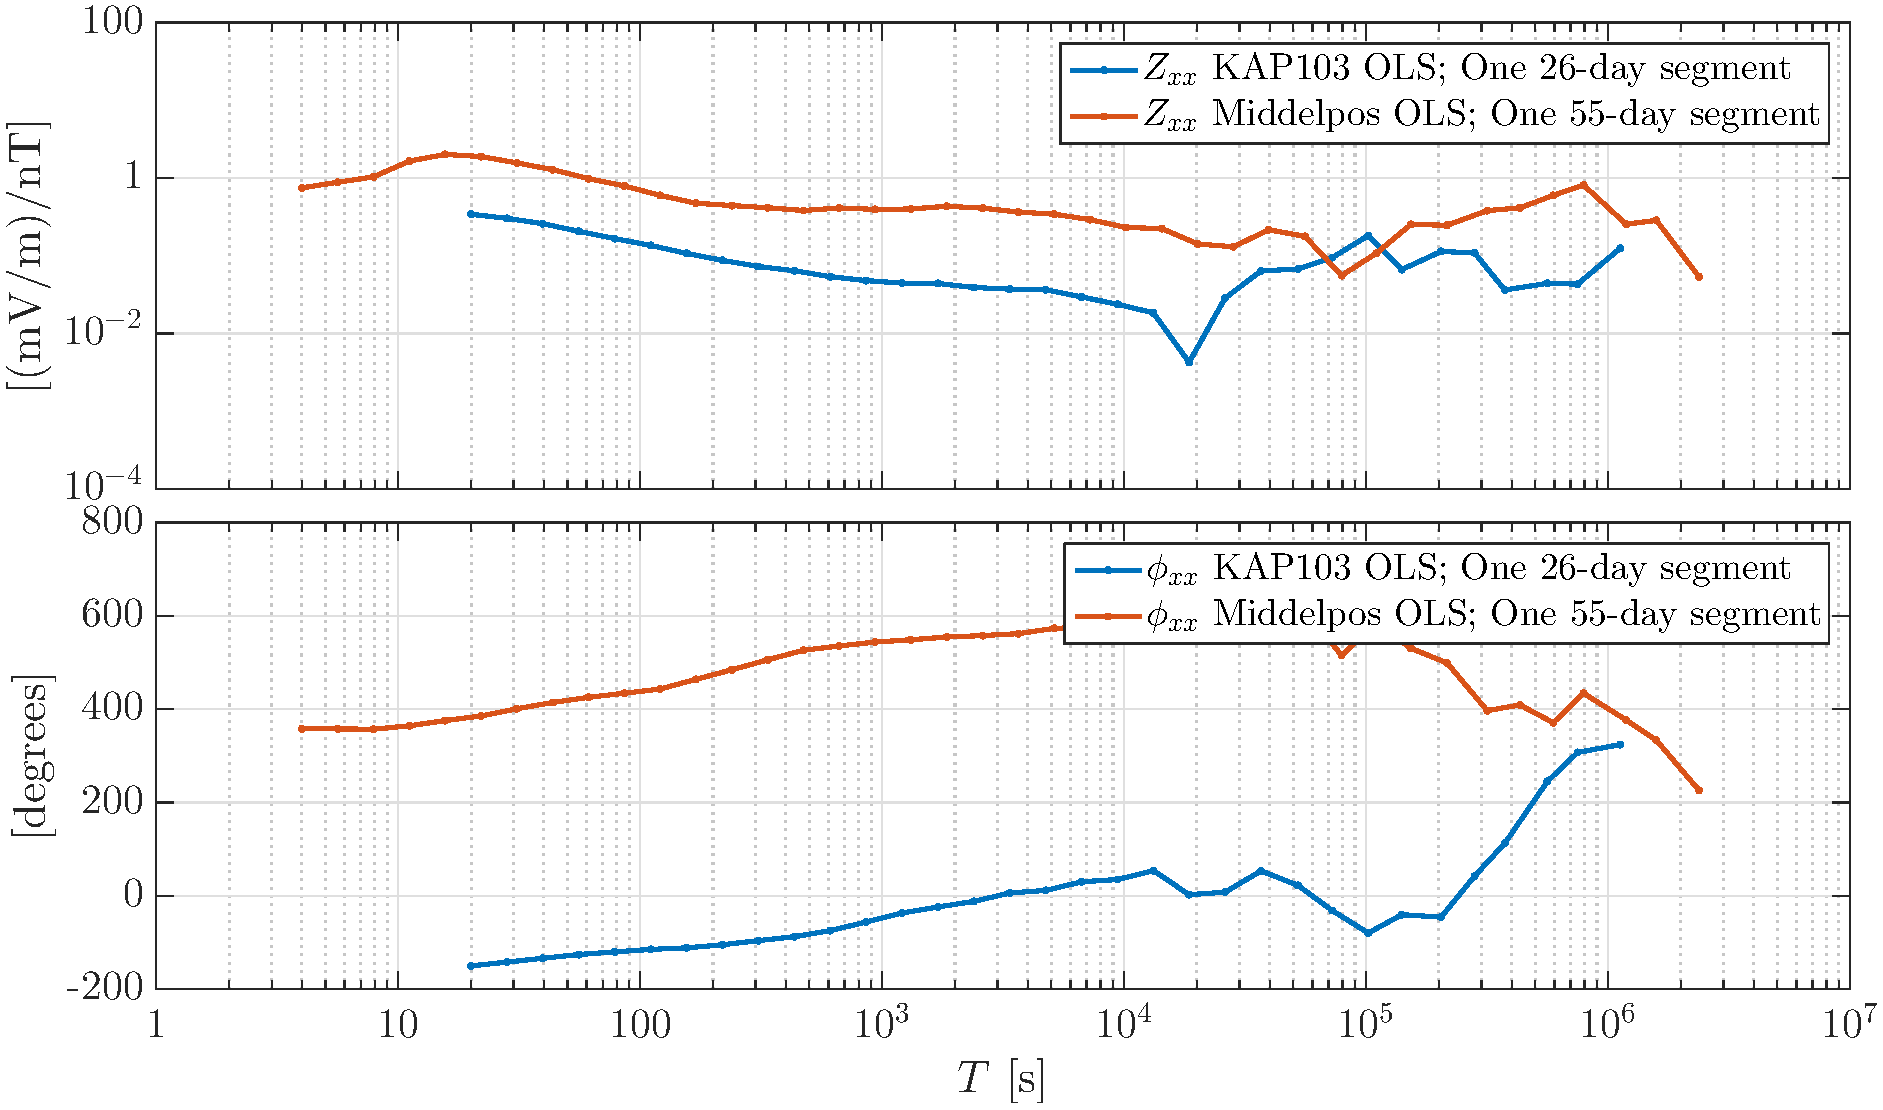
\includegraphics[width=\textwidth]{figures/KAP103_Middelpos/Z_xx_Magnitude_Phase.pdf}
\caption{}
\label{fig:universe}
\end{figure}

\begin{figure}[h!]
\centering
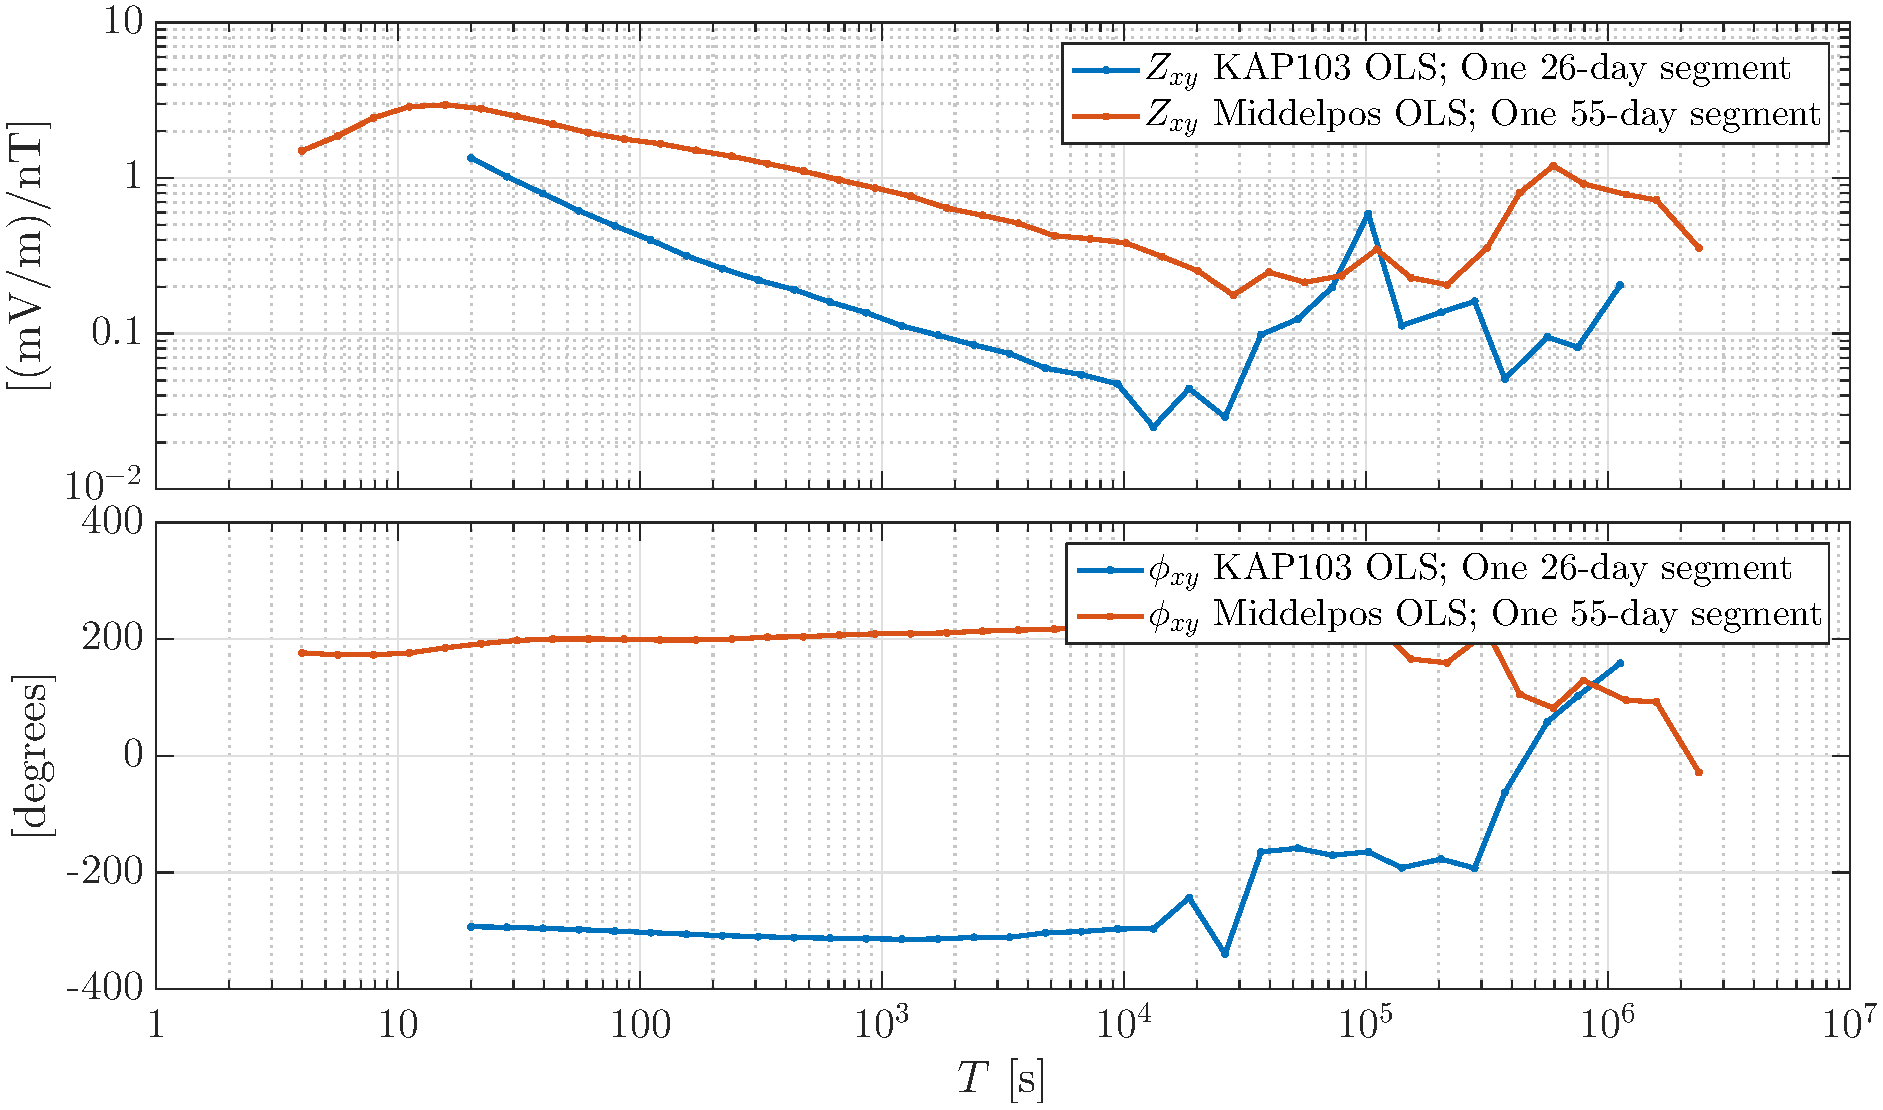
\includegraphics[width=\textwidth]{figures/KAP103_Middelpos/Z_xy_Magnitude_Phase.pdf}
\caption{}
\label{fig:universe}
\end{figure}

\clearpage

\begin{figure}[h!]
\centering
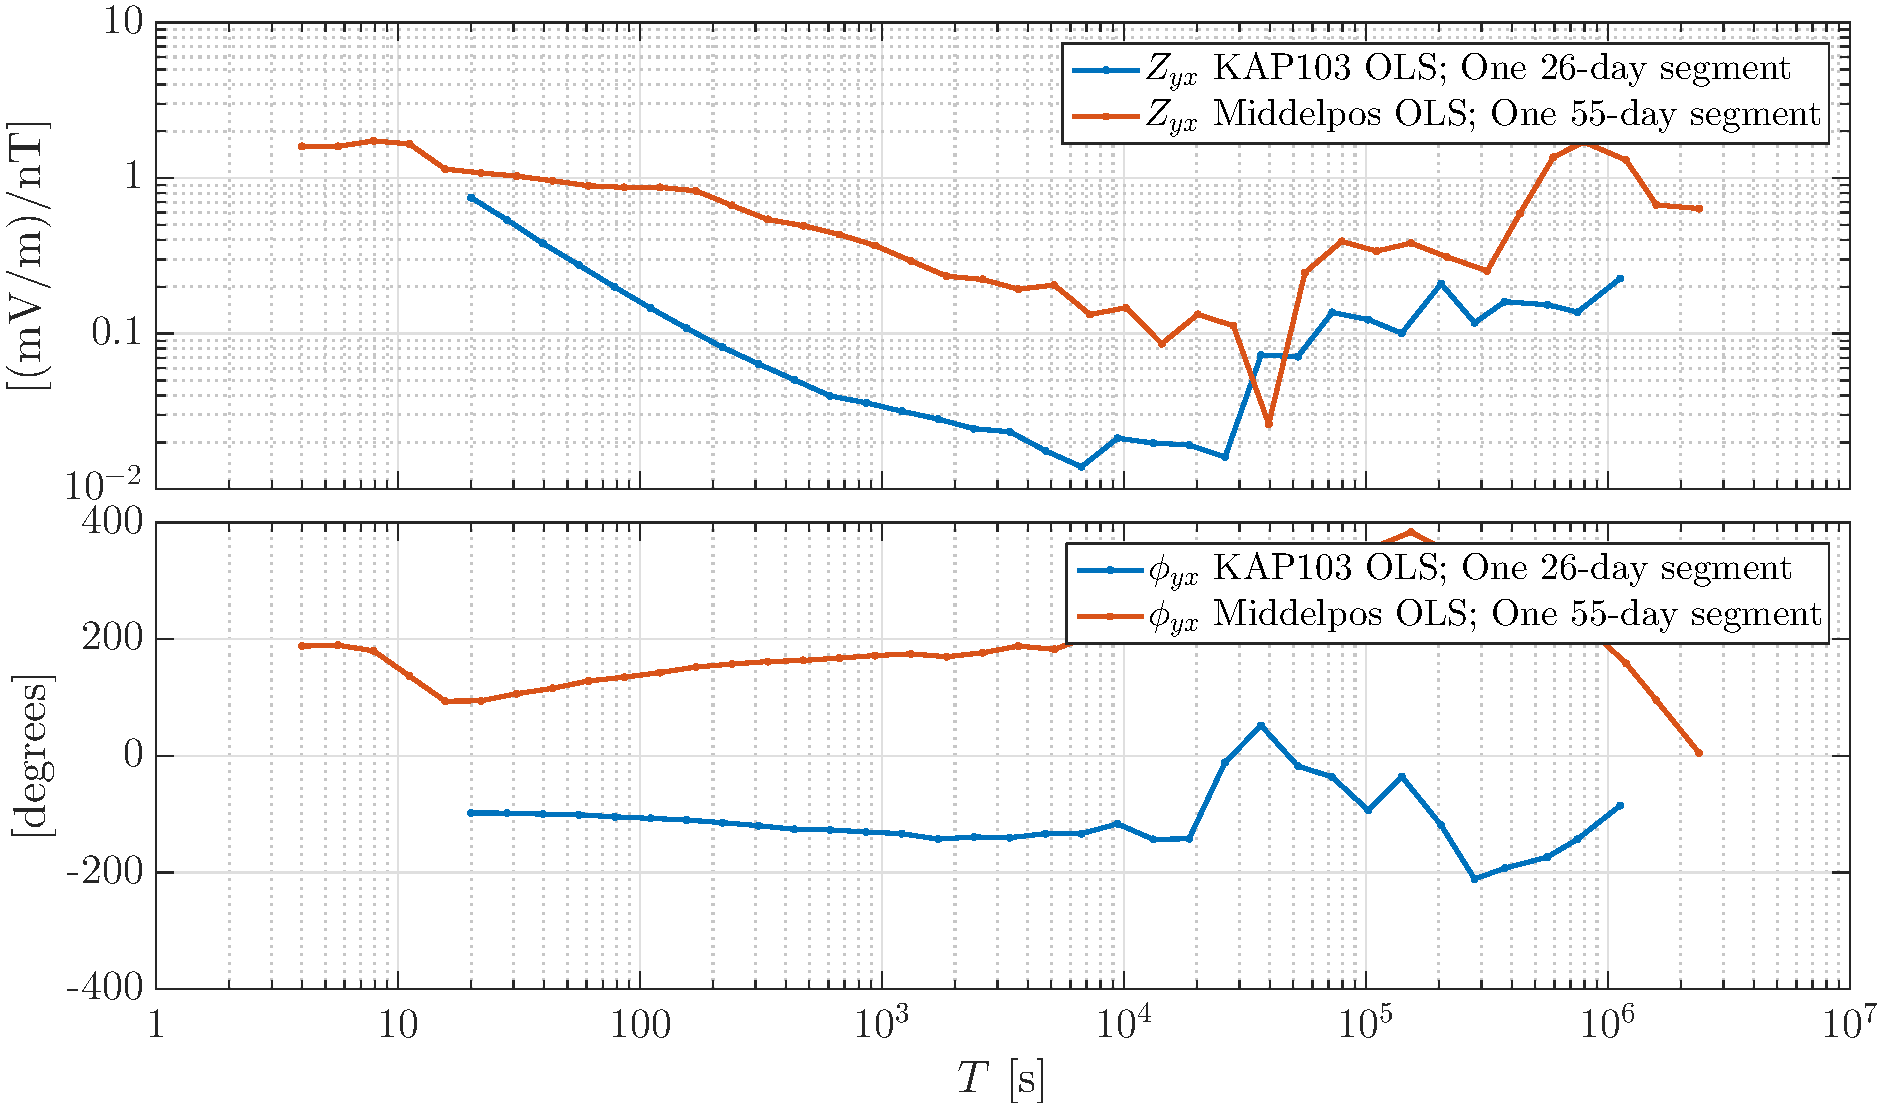
\includegraphics[width=\textwidth]{figures/KAP103_Middelpos/Z_yx_Magnitude_Phase.pdf}
\caption{}
\label{fig:universe}
\end{figure}

\begin{figure}[h!]
\centering
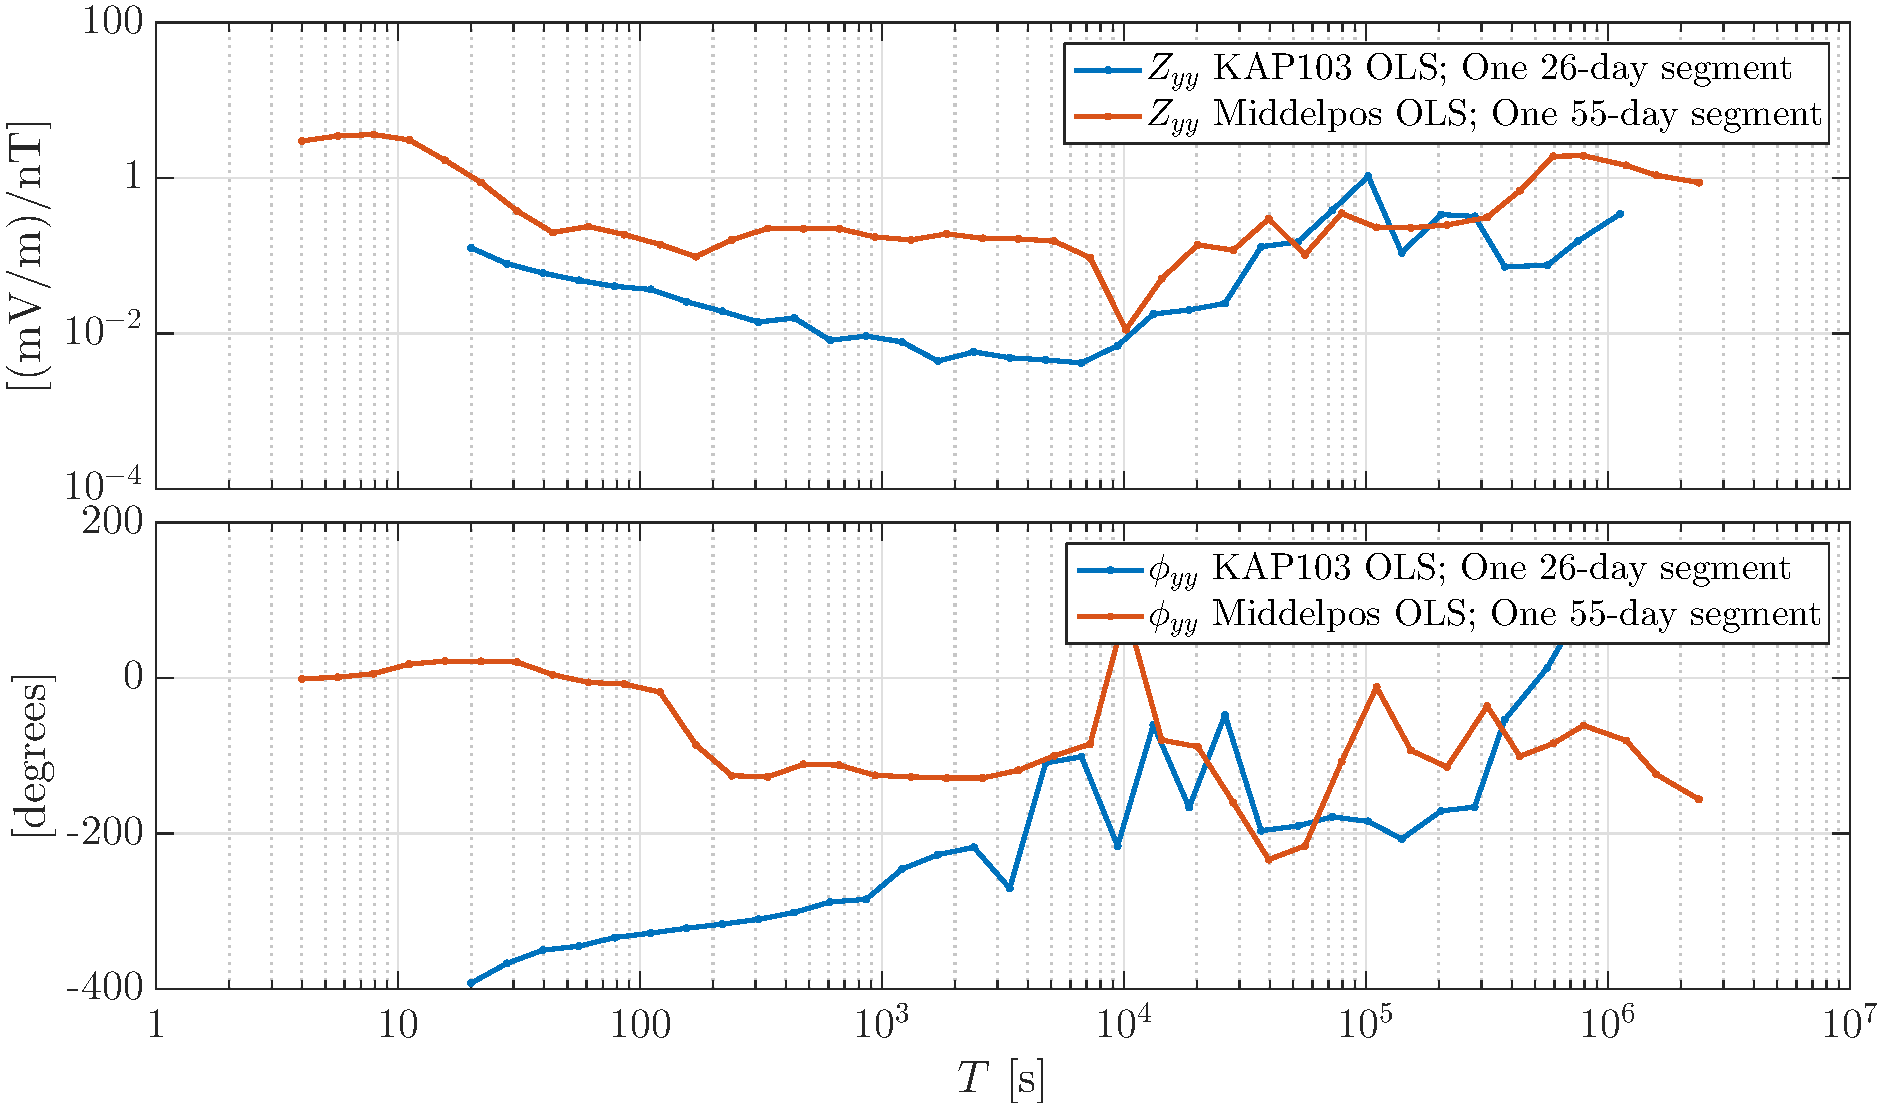
\includegraphics[width=\textwidth]{figures/KAP103_Middelpos/Z_yy_Magnitude_Phase.pdf}
\caption{}
\label{fig:universe}
\end{figure}

\end{document}
